\section{Analisis Rancangan Solusi}
\label{sec:analisis-rancangan-solusi}

Berdasarkan beberapa pendekatan yang telah dijelaskan pada \ref{sec:analisis-solusi}, Membuat sistem \textit{remote deployment}, yang dirancang untuk provisioning skala besar dari aplikasi pada perangkat \textit{IoT} yang terbatas sumber daya, menggunakan Kubernetes menjadi solusi yang akan digunakan karena beberapa keuntungan yang tidak dimiliki oleh pendekatan lain. Kubernetes, sebagai sistem orkestrasi kontainer yang matang dan luas digunakan, menawarkan fitur dan kemampuan yang cocok untuk mengatasi tantangan yang dihadapi dalam lingkungan \textit{IoT} yang heterogen dan terdistribusi terutama dalam masalah skalabilitas, \textit{ready to use}, serta memakan waktu yang minimal sehingga solusi ini merupakan solusi paling feasible yang dapat diimplementasikan

\subsection{Analisis kebutuhan sistem}

Sebelum sistem dibuat, pertama tama akan dibuat dan dicari kebutuhan sistem yang diperlukan. Kebutuhan sistem akan dibagi menjadi kebutuhan fungsional dan non-fungsional.

\subsubsection{Deskripsi sistem}
Sistem yang akan dibuat merupakan sebuah sistem yang dapat melakukan sebuah aksi, command, ataupun \textit{remote deployment} ke perangkat yang terhubung ataupun ke sebagian perangkat yang diinginkan. Sistem memiliki tiga komponen utama, dashboard atau \textit{entrypoint}, database, dan kubernetes sebagai orkestrator. Kubernetes nantinya akan terhubung ke kluster yang diinginkan untuk melakukan sebuah aksi,command, ataupun melakukan proses \textit{remote deployment} ke masing masing perangkat yang terhubung.

\begin{figure}[h]
  \centering
  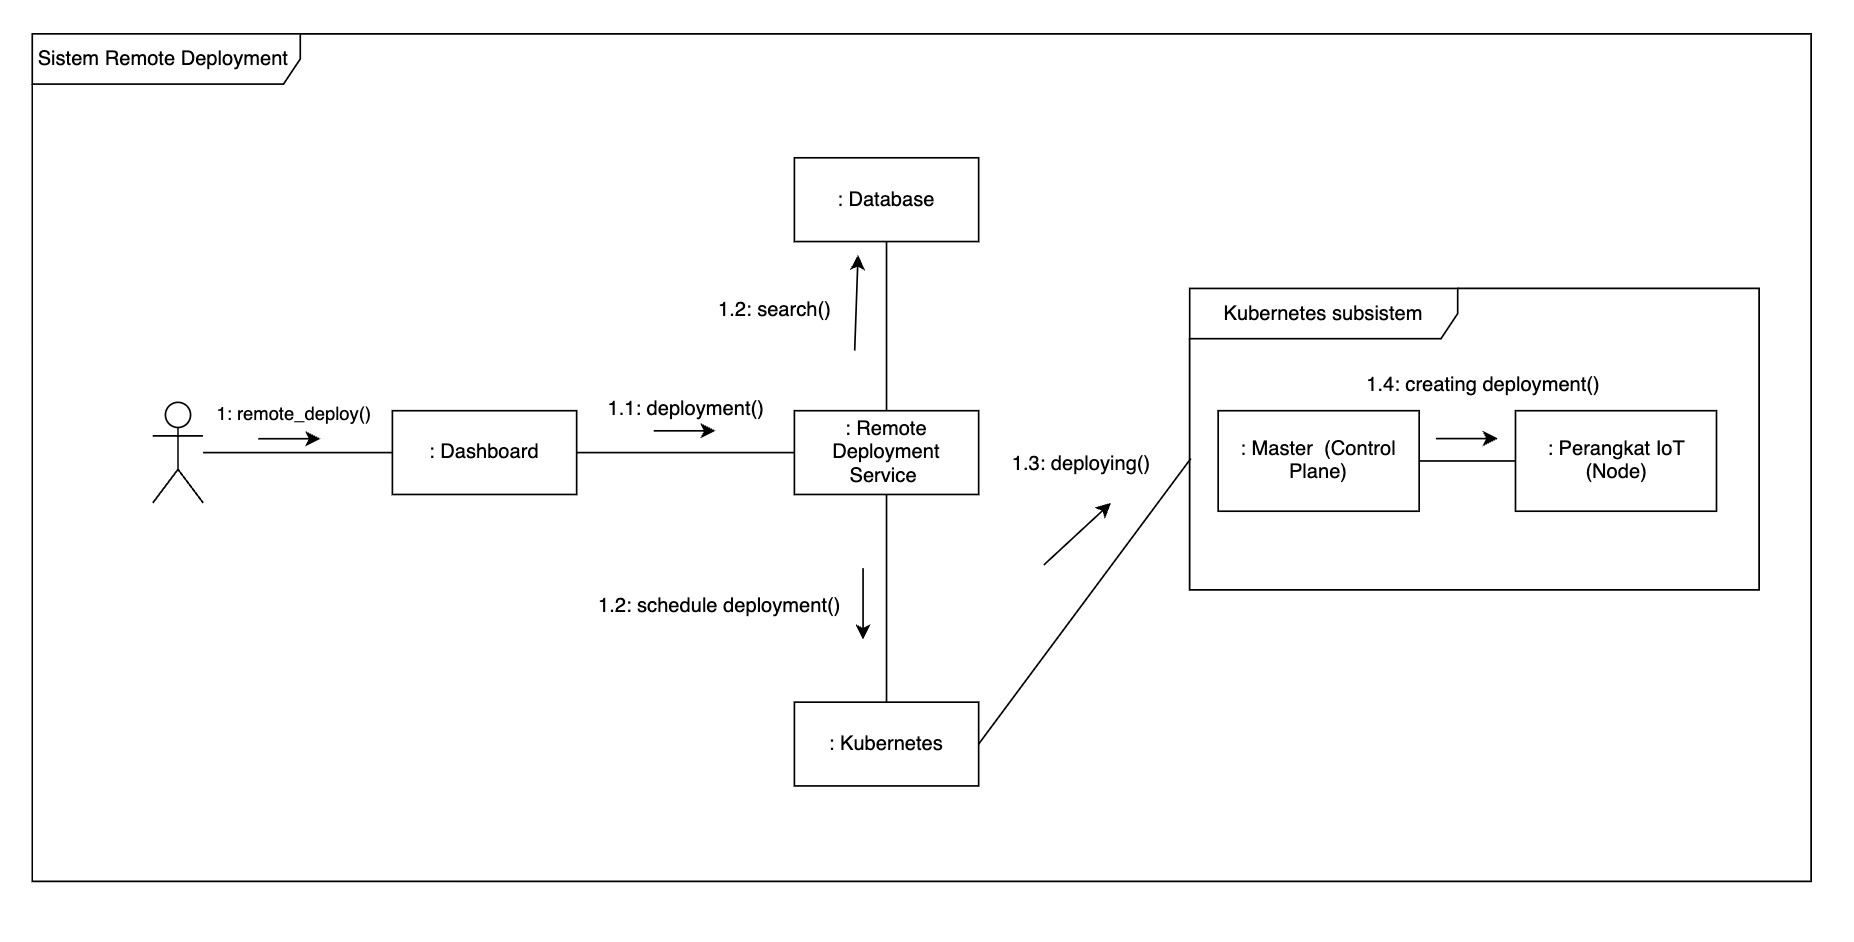
\includegraphics[width=1\textwidth]{resources/chapter-3/gambaran-umum-arsitektur-updated.jpg}
  \caption{Gambaran Umum Arsitektur}
  \label{fig:gambaran-umum-arsitektur}
\end{figure}

\pagebreak

\subsubsection{Kebutuhan Fungsional}
Berikut merupakan kebutuhan fungsional dari sistem yang akan dibuat, agar lebih jelas kebutuhan fungsional dibuat ke dalam bentuk tabel di bawah ini. Semua kebutuhan fungsional akan memiliki ID yang diawali dengan huruf F lalu diikuti dengan dua angka.
\begin{table}[h]
  \caption{Kebutuhan Fungsional}
  \label{tab:kebutuhan-fungsional}
  \centering
  \begin{tabular}{|c|p{4.5cm}|p{4.5cm}|}
    \hline
    ID  & Kebutuhan                                                                         & Penjelasan                                                                                                 \\
    \hline
    F01 & Sistem dapat meregistrasi perangkat \textit{IoT}                                  & User dapat melakukan registrasi perangkat \textit{IoT} untuk dimasukkan ke dalam database sistem           \\
    \hline
    F02 & Sistem dapat melihat list perangkat                                               & User dapat melihat seluruh pernagkat yang telah teregistrasi                                               \\
    \hline
    F03 & Sistem dapat melakukan \textit{remote deployment} kepada perangkat yang terhubung & User dapat melakukan sebuah aksi melalui sistem untuk mengoperasikan perangkat \textit{IoT} yang terhubung \\
    \hline
  \end{tabular}
\end{table}


\subsubsection{Kebutuhan Non-Fungsional}
Berikut merupakan kebutuhan non fungsional dari sistem yang akan dibuat, agar lebih jelas kebutuhan non fungsional dibuat ke dalam bentuk tabel di bawah ini. Semua kebutuhan non-fungsional memiliki ID NF lalu diikuti oleh dua angka
\begin{table}[h]
  \caption{Kebutuhan Non-Fungsional}
  \label{tab:kebutuhan-non-fungsional}
  \centering
  \begin{tabular}{|c|p{4.5cm}|p{4.5cm}|}
    \hline
    ID   & Parameter    & Kebutuhan                                                  \\
    \hline
    NF01 & Availability & Sistem akan terus menerus beroperasi 7 hari
    perminggu, 24 jam per hari tanpa gagal                                           \\
    \hline
    NF02 & Security     & Sistem akan menjamin keamanan dari masing masing perangkat \\
    \hline
    NF02 & Security     & Sistem akan menjamin keamanan dari masing masing perangkat \\
    \hline
  \end{tabular}
\end{table}

\subsection{Rancangan Sistem}
Seperti yang telah digambarkan pada gambar \ref{fig:gambaran-umum-arsitektur}, terdapat tiga komponen utama yang menjadi dasar dari sistem, selain itu terdapat beberapa tambahan berupa perangkat \textit{IoT} yang akan dijadikan node pada \textit{cluster kubernetes}.
